\chapter{Auswahl der Hardware}
Die Auswahl von Hardware mit ARM-Prozessoren ist extrem gross.
Ende September 2016 sind bereits über 86 Milliarden ARM-basierte Prozessoren verkauft worden.\footnote{\ \ Direkter Link: \ \ \ \ \ \ \ \ \ https://www.arm.com/-/media/arm-com/news/ARM-media-fact-sheet-2016.pdf\\ Archivierter Link: \ \ \ https://web.archive.org/web/20180808122231/https://www.arm.com/-/media/arm-com/news/ARM-media-fact-sheet-2016.pdf}
Diese Zahl reflektiert zwar nicht direkt die Diversität der verschiedenen Prozessoren, aber sie zeigt recht gut wie enorm weit ARM-Prozessoren verbreitet sind.

In diesem Kapitel soll aus dem riesigen Angebotsdschungel die richtige Hardware ausgewählt werden, auf der diese Arbeit aufbauen kann.
Die ausgewählte Hardware soll nicht nur für diese Arbeit genutzt werden, sondern später auch für den Robotik-Unterricht.
Zusätzlich sollte der Prozessor auch leistungsstark und flexibel genug sein, um ihn, oder eine Variante aus der gleichen Familie, in anspruchsvollen Robotikprojekten verwenden zu können.
%TODO extrem weit verbreitet
%TODO warum muss hw in dieser arbeit gewählt werden

%TODO prozeossor und board muss ausgewählt werden
%TODO ökosystem?

\section{Soll-Kriterien und Muss-Kriterien bei der Auswahl der Hardware}
Für die Hardware sind folgende Soll-Kriterien und Muss-Kriterien ermittelt worden.


\subsection{Muss-Kriterien}
\begin{itemize}
\item Systemebene
	\begin{itemize}
	\item FPGA: Der Prozessor muss mit einem FPGA kommunizieren können.
	\item Hardware Debugger: Der Prozessor muss für die Entwicklung von \textit{deep} einen Hardware Debugger, wie beispielsweise das BDI3000, von Abatron unterstützen. 
	\item Günstiger Programmierer: Wenn zusätzliche Hardware benötigt wird, um die \textit{deep}-Applikation auf das Target zu schreiben, dann muss diese möglichst günstig sein.
	\item Grosses Ökosystem: Das ausgewählte Produkt muss von einem grossen Ökosystem unterstützt werden. Aussterbende Produkte oder Nischenprodukte sind nicht akzeptabel.
	\item Als fertiges Modul erhältlich: Für den Unterricht ein eigenes PCB entwickeln und herstellen ist keine Option.
	%TODO synonym einbettbar:
	\item Einbettbar: Der Prozessor muss auch bei einem selbstentwickelten PCB verwendet werden können. Wahlweise als SOM (\textit{System On Module}) oder direkt als Prozessor im eigenen Package.
	\item Die Hardware muss noch lange erhältlich bleiben.
	\item FPU (\textit{Floating Point Unit}): Für Gleitzahlenarithmetik.
	\item Netzwerkschnitstelle: RJ-45 inklusive MAC (\textit{Media Access Control}) und \textit{Magnetics}.
	\item USB: USB Schnittstelle als Host und als Slave.
	\item Flash: Mehr als 50kByte Flash.
	\item RAM: Mehr als 100kByte RAM.
	\end{itemize}
\item Prozessorebene
	\begin{itemize}
	\item ARMv7: Der Prozessor muss auf einer ARMv7 ISA (\textit{Instruction Set Architecture}) basieren.
	\item ARM Instruktionen: Der Prozessor muss ARM Instruktionen unterstützen. \textit{Thumb} Instruktionen sind nicht ausreichend.
	\end{itemize}
\end{itemize}


\subsection{Soll-Kriterien}
\begin{itemize}
\item Systemebene
	\begin{itemize}
	%TODO synonym einbettbar:
	\item Einfach einbettbar: Der Prozessor ist als Prozessormodul erhältlich, sodass das Design von einem selbstentwickelten PCB einfacher wird.
	\item Günstiger Hardware Debugger: Der Hardware Debugger kann auch für die Applikationsentwicklung mit \textit{deep} eingesetzt werden.
	\item Möglichst schneller Download der Applikation.
%TODO	\item Überdimensionierte HW
	\end{itemize}
\item Prozessorebene
	\begin{itemize}
	\item Memory Mapped Bus für FPGA Schnittstelle.
	\item FPU unterstützt \textit{Double Precision}.
	\item Integerdivision
	\item Prozessortakt über 500MHz.
	\end{itemize}
\end{itemize}


\section{Was ist ein Hardware Debugger}
Der Begriff \textit{Hardware Debugger} ist nicht eindeutig definiert.
Im einfachsten Fall kann ein Hardware Debugger nur einen \textit{Boundary Scan} durchführen, wie es ursprünglich für JTAG vorgesehen war.
Bei \textit{Boundary Scan} können die I/O Pins von einem Prozessor gelesen und auch gesetzt werden.
Mit solch einem Scan kann während der Produktion bei den bestückten PCBs überprüft werden, ob alle Lötstellen Kontakt herstellen und dabei keine Kurzschlüsse bilden.
Für diesen Scan wird der Prozessor-Kern nicht verwendet, sondern eine separate Peripherie im Prozessor.
Über das JTAG-Interface kann der Scan ausgeführt werden, ohne dass eine Applikation auf dem Prozessor ausgeführt werden muss.

Moderne Prozessoren erweitern diese grundlegendsten Funktionen mit einigen sehr hilfreichen Features.
% Moderne Prozessoren haben noch viel mehr Funktionen.
So bieten ARM-Prozessoren mit der \textit{CoreSight}-Technologie noch viel mehr als nur einen \textit{Boundary Scan}.
% TODO besserer Satz
Die untenstehende Liste zeigt einige Funktionen dieser Technologie, aber nicht alle.
Die für diese Arbeit relevanten Funktionen sind \textbf{fett} geschrieben.

\begin{itemize}
	\item \textbf{Prozessor Register lesen und schreiben}
	\item \textbf{RAM lesen und schreiben}
	\item \textbf{Externer Flash Speicher lesen und schreiben} 
	\item \textbf{Hardware Breakpoint auf den Program Counter} 
	\item Hardware Breakpoint auf einer Speicherstelle (Watchpoint)
	\item Debug Trace (ETM Program Trace) 
	\item Debug Trace Buffer
\end{itemize}

Da ein Hardware Debugger keine funktionsfähige Software auf dem Prozessor benötigt, kann er auch gut verwendet werden, um die grundlegendsten Funktionen, wie beispielsweise den Bootvorgang, vom \textit{deep} Laufzeit System zu entwickeln.




\section{Übersicht über die ARM Mikroarchitekturen}
In diesem Kapitel werden die verschiedenen ARM-Architekturen untersucht und beurteilt.
Tabelle \ref{t-uebersichtARMMikroarchitekturen} fasst alle Vor- und Nachteile zusammen.

\subsection{Cortex-A}
Prozessoren der Cortex-A Familie sind gut geeignet für die Verwendung mit einem vollen Betriebssystem, wie Windows, Linux oder Android.
Cortex-A Prozessoren bieten den umfangreichsten Support für externe Peripherien, wie USB, Ethernet und RAM.
Sie sind auch die leistungsstärksten ARM-Cortex Prozessoren.

\subsection{Cortex-R}
Cortex-R Prozessoren werden entwickelt für Echtzeitanwendungen und sicherheitskritische Applikationen, wie Festplattenkontroller und medizinische Geräte.
Sie sind normalerweise nicht mit einer MMU (\textit{Memory Management Unit}) ausgerüstet.
% und können deshalb nich mit einem Linux oder Windows verwendet werden.
Mit einer Taktrate von über 1GHz und einem sehr schnellen Interruptverhalten eignen sich Prozessoren mit einem Cortex-R sehr gut, um auf externe Stimuli schnell zu reagieren.

\subsection{Cortex-M}
Die Prozessoren aus der Cortex-M Familie sind mit einer Taktrate um 200Mhz relativ langsam.
Sie sind sehr stromsparend und durch die kurze Pipeline haben sie eine deterministische und kurze Interruptverzögerung.
Die Prozessoren aus der Cortex-M Reihe unterstützen aber nur die Thumb-Instruktionen und kommen deshalb nicht in Frage.

\subsection{ARM-Prozessoren ausserhalb der Cortex Reihe}
Seit 2004 werden die meisten Kerne in eine der Cortex-Familien eingeteilt.
Ältere Kerne, sogenannte \textit{''Classic cores''}, haben Namen wie z.b. ARM7 oder ARM1156T2F-S.
Da solche Designs meist aus einer Zeit vor 2004 stammen, gilt das Design als veraltet und wird bei dieser Arbeit nicht berücksichtigt.

\subsection{Fazit über die Wahl der ARM-Mikroarchitekturen}
Die Prozessoren, die auf der Cortex-A Mikroarchitektur basieren, bieten die grösste Flexibilität.
Zusätzlich ist das Angebot bei den Cortex-A-Prozessoren am grössten.
Die anderen Cortex-Reihen bieten keine Vorteile, die für dieses Projekt von Nutzen sind.
Aus diesen Gründen wird die Auswahl auf die Prozessoren aus der Cortex-A-Reihe begrenzt.

\begin{table}[]
\centering
\label{t-uebersichtARMMikroarchitekturen}
\begin{tabular}{|l|l|l|}
\hline
\textbf{}  & \textbf{Vorteile}                                                                                                                                                                                                                                    & \textbf{Nachteile}                                                                                                                                                                             \\ \hline
\textbf{A} & \begin{tabular}[c]{@{}l@{}}* Sehr leistungsstark\\ * Support für vollwertige Betriebssysteme\\ * Grosse Variation erhältlich (energiesparend /\\  sehr leistungsstark)\\ * Reichhaltiger Funktionsumfang\\ * NEON und FPU-Unterstützung\end{tabular} & \begin{tabular}[c]{@{}l@{}}* Langsamer Context-Switch\\ * Relativ hoher Stromverbrauch\\ * Relativ teuer\\ * Mit GPU erhältlich\\ * Keine DSP-Unterstützung\\ * Keine HW-Division\end{tabular} \\ \hline
\textbf{R} & \begin{tabular}[c]{@{}l@{}}* Sehr gut geeignet für Echtzeitanwendungen\\ * Sehr schneller Context-Switch\\ * DSP-Unterstützung\end{tabular}                                                                                                           & \begin{tabular}[c]{@{}l@{}}* Kleiner Funktionsumfang\\ * Nicht so leistungstark wie Cortex A\\ * Keine Linux-Unterstützung\end{tabular}                                                        \\ \hline
\textbf{M} & \begin{tabular}[c]{@{}l@{}}* Sehr schneller Context-Switch\\ * Sehr energiesparend\\ * DSP-Unterstützung\end{tabular}                                                                                                                                & \begin{tabular}[c]{@{}l@{}}* Geringe Rechenleistung\\ * Keine Linux-Unterstützung\\ * Unterstützt nur Thumb-Instruktionen\end{tabular}                                                         \\ \hline
\end{tabular}
\caption{Übersicht ARM Mikroarchitekturen}
\end{table}



\section{Anbindung des FPGAs an den Prozessor}
FPGAs haben typischerweise einen sehr hohen \textit{Pin-Count} und werden in \textit{BGA-Packages} ausgeliefert.

Es gibt verschiedene Möglichkeiten, wie ein FPGA mit einem Prozessor verbunden werden kann.
Die Vor- und Nachteile der verschiedenen Bauarten werden in diesem Kapitel abgewogen und in der Tabelle \ref{t-uebersichtBauformen} zusammengefasst.
Bild \ref{fig:anbindungFPG} gibt eine schematische Übersicht über die verschiedenen Bauarten.

% Um ein FPGA an einen Prozessor anzubinden kann eine serielle und auch parallele Kommunikation verwendet werden.


% Ein moderner Prozessor ist ein sehr komplexes elektronisches Bauteil welches zusätzliche Peripherie für beispielsweise Stromversorgung und auch diverse I/Os.
% Die Ethernet Schnittstelle braucht neben der RJ-45 Buchse auch noch Signaltransformatoren, sogenannte Magneticts.
% % % TODO doofer satz
% % Auch wenn die Physikalische Anbindung der Ethernet Schnittstelle nicht ganz trivial ist, ist die Anbindung von RAM sehr viel anspruchsvoller.

% % Externer RAM muss über sehr viele Leitungen, welche alle gleich lang sein müssen und auch von der elektrischen Impedanz enge Parameter erfüllen müssen, an den Prozessor angeschlossen werden.
% % Diese Ansprüche erfordern sehr hohe Fachkenntnisse vom Designer.



\begin{figure}[htbp]
	\centering
		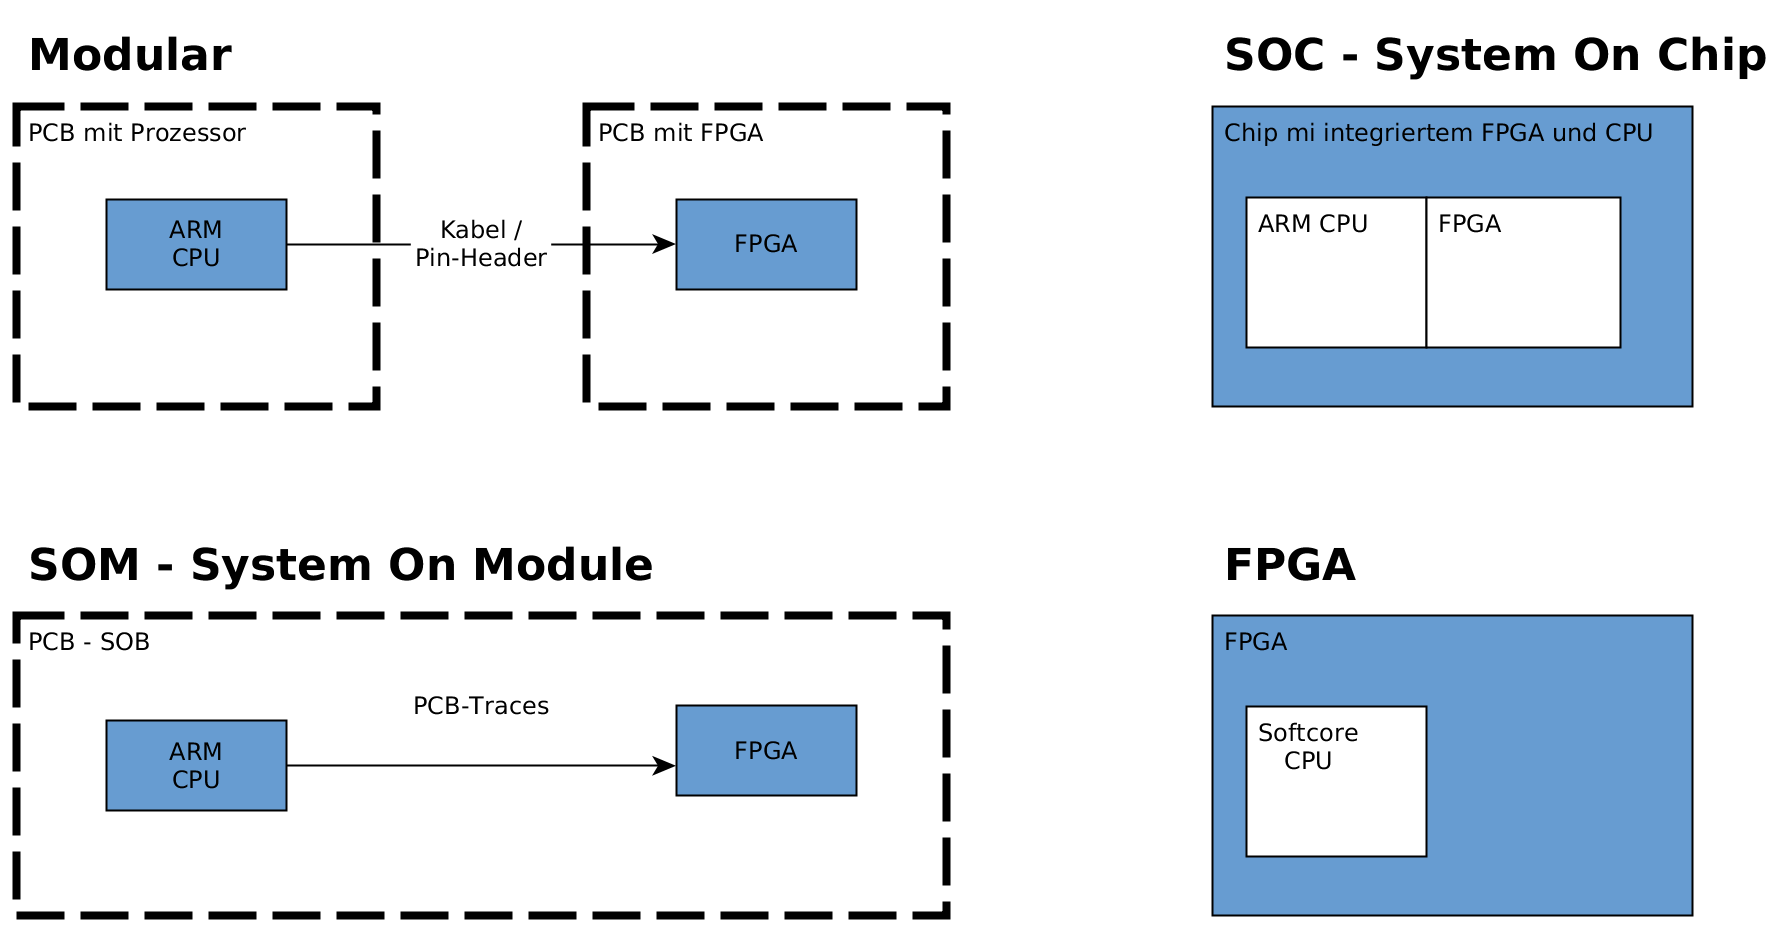
\includegraphics[width=\textwidth,height=\textheight,keepaspectratio]{graphs/bauformen.png}
	\caption[]{Mögliche Anbindungen des FPGA an die CPU}
	\label{fig:anbindungFPG}
\end{figure}
% \FloatBarrier

\subsection{FPGA als Zusatzplatine zum Prozessorboard - Bauweise ''Modular''}
Das \textit{''FPGA Development Board CAPE for the BEAGLEBONE''}\footnote{\ \ Direkter Link: \ \ \ \ \ https://www.element14.com/community/docs/DOC-69215/l/fpga-development-board-cape-for-the-beaglebone\\ Archivierter Link: \ \ \ https://web.archive.org/save/https://www.element14.com/community/docs/DOC-69215/l/fpga-development-board-cape-for-the-beaglebone}  ist eine Aufsteckplatine für den \textit{Beaglebone Black}.
Wenn sie auf den \textit{Beaglebone Black} aufgesteckt wird, erweitert sie den ARM-basierten Linux PC um einen \textit{''Spatran 6 LX9''} FPGA, inklusive einiger I/O-Peripherien und SDRAM.

\textit{Vorteile:}
\begin{itemize}
	\item Relativ günstig.
	\item Funktioniert ''Out of the Box''
	\item Schnelles GPMC-Interface (General-Purpose Memory Controller) zwischen Prozessor und FPGA.
\end{itemize}

\textit{Nachteile:}
\begin{itemize}
	\item Verwendet ein modifiziertes Linux-Image, das LOGI-Image.
	\item Der eMMC (Embedded Multi Media Card) Speicher des Beaglebone kann nicht gleichzeitig mit dem GPMC verwendet werden.
	\item Die Verfügbarkeit vom Cape ist nicht garantiert.
	\item Nur ein FPGA und Prozessor erhältlich.
\end{itemize}

Eine modulare Bauweise ist grundsätzlich sehr flexibel.
Leider sind auf dem Markt nur sehr wenige verschiedene Module zu finden.
So ein kleines Angebot disqualifiziert diese Bauweise.


\subsection{FPGA auf dem gleichen Modul wie der Prozessor (System On Module) - Bauweise ''SOM''}
Bei einem SOM (System On Module) ist die CPU und auch der FPGA auf dem gleichen PCB-Modul verbaut.
Dadurch kann der Hersteller auf dem Modul ein Bus mit kontrollierter Impedanz implementieren.
Dies ermöglicht eine sehr hohe Bandbreite bei der Kommunikation zwischen der CPU und dem FGPA.
Das Modul benötigt ein zusätzliches PCB, ein Basisboard, in dem es eingebettet werden kann.
Oft existieren Experimentierboards mit einer grossen Zahl an unterschiedlichen I/O-Möglichkeiten, die gebrauchsfertig gekauft werden können.
Für eine spezifische Anwendung muss ein solches Basisboard für das SOM selbst designed werden, weil ein Experimentierboard oft zu gross ist, oder nicht die benötigte Peripherie enthält.
Da neben dem FPGA auch High-Speed-Peripherie, wie z.B. RAM auf dem Modul verbaut ist, kann beim Basisboard oft auf die aufwändige Entwicklung von High-Speed-PCB-Traces verzichtet werden.


Es hat sich gezeigt, dass es nur zwei Anbieter SOM mit FPGA produzieren.
Nur die beiden Anbieter \textit{solectrix}\footnote{\ \ Direkter Link: \ \ \ \ \ \ \ \ \ https://www.solectrix.de/de/sxom-module\\ Archivierter Link: \ \ \ https://web.archive.org/save/https://www.solectrix.de/de/sxom-module} und \textit{OposSom}\footnote{\ \ Direkter Link: \ \ \ \ \ \ \ \ \ http://www.opossom.com/english/products-processor\_boards-apf6\_sp.html\\ Archivierter Link: \ \ \ https://web.archive.org/save/http://www.opossom.com/english/products-processor\_boards-apf6\_sp.html} scheinen solche Module zu verkaufen.

Weil die Auswahl für SOMs sehr klein ist wurde diese Bauform nicht mehr weiter verfolgt.

 
\subsection{FPGA im gleichen Gehäuse wie der Prozessor (System On Chip) - Bauweise ''SOC''}
Seit einigen Jahren werden Produkte verkauft, die eine programmierbare Logik (FPGA) und auch eine dedizierte CPU in einem Chip-Gehäuse verbaut haben.
Da der FPGA und auch die CPU im selben Gehäuse verbaut sind, ist eine sehr schnelle, integrierte Kommunikation zwischen CPU und FPGA möglich.

Die beiden grossen FPGA-Hersteller Altera und auch Xilinx bieten beide mehrere Produkte als eine SOC Lösung an.
Die Produkte von Altera sind aber deutlich teurer als die Chips von Xilinx.
Besonders die Evaluierungsboards von Altera sind sehr teuer.

Bei der Produktfamilie Zynq von Xilynx gibt es ein breites Angebot von SOCs und auch von Experimentierboards.
Das Experimentierboard \textit{''Zybo''} wird sogar schon im Unterricht der NTB für die Entwicklung von VHDL genutzt.



\subsection{ARM als Softcore in FPGA - Bauweise ''FPGA''}
In FPGAs können Prozessoren als sogenannte \textit{Softcores} implementiert werden.
Dabei wird ein Teil der FPGA-Gates so konfiguriert, dass sie wie ein Mikroprozessor verwendet werden können.

Es existieren aber nur Designs für einfachere Mikroprozessoren, da komplexe Prozessoren viel zu viele Gates benötigen, um ökonomisch sinnvoll zu sein.
ARM-Prozessoren der Cortex-A-Familie sind sehr komplex und nicht als FPGA-Softcores erhältlich.
Von der ARM-Cortex-Familie sind nur Cortex-M0 und Cortex-M1 erhältlich.
Diese Cores sind aber kostenpflichtig und nicht Open Source.

Weil keine Cortex-A-Cores erhältlich sind und alle anderen ARM-Cores kostenpflichtig sind, wird diese Bauweise nicht mehr weiter verfolgt.


\begin{table}[htbp]
\centering
\begin{tabular}{|l|l|l|}
\hline
\textbf{Bauweise} & \textbf{Vorteile}                                                                                                                      & \textbf{Nachteile}                                                       \\ \hline
\textbf{Modular}  & \begin{tabular}[c]{@{}l@{}}* Günstig wenn nur Prozessor verwendet wird\\ * Unterschiedliche FPGAs können verwendet werden\end{tabular} & \begin{tabular}[c]{@{}l@{}}* Datenbus evt. nicht Memory \\mapped    \end{tabular}                                  \\ \hline
\textbf{SOB}      & \begin{tabular}[c]{@{}l@{}}* Sauberes, abgeschlossenes System\end{tabular} & * FPGA ist fix                                                           \\ \hline
\textbf{SOC}      & \begin{tabular}[c]{@{}l@{}}* Potenziell sehr schnelle Datenverbindung\\ \ \ \ zwischen FPGA und Prozessor\\ * Sauberes, abgeschlossenes System\end{tabular}                       & \begin{tabular}[c]{@{}l@{}}* FPGA ist fix\\ * Relativ teuer\end{tabular} \\ \hline
\textbf{FPGA}     & * Flexibel                                                                                                                             & * Sehr teuer                                                             \\ \hline
\end{tabular}
\label{t-uebersichtBauformen}
\caption{Übersicht Bauformen}
\end{table}

%\section{Cortex-M}
%\textbf{Cortex-M0}
%A very small processor (starting from 12K gates) for low cost, ultra low power microcontrollers and deeply embedded applications
%
%\textbf{Cortex-M0+}
%The most energy-efficient processor for small embedded system. Similar size and programmer’s model to the Cortex-M0 processor, but with additional features like single cycle I/O interface and vector table relocations
%
%\textbf{Cortex-M1}
%A small processor design optimized for FPGA designs and provides Tightly Coupled Memory (TCM) implementation using memory blocks on the FPGAs. Same instruction set as the Cortex-M0
%
%\textbf{Cortex-M3}
%A small but powerful embedded processor for low-power microcontrollers that has a rich instruction set to enable it to handle complex tasks quicker. It has a hardware divider and Multiply-Accumulate (MAC) instructions. In addition, it also has comprehensive debug and trace features to enable software developers to develop their applications quicker
%
%\textbf{Cortex-M4}
%It provides all the features on the Cortex-M3, with additional instructions target at Digital Signal Processing (DSP) tasks, such as Single Instruction Multiple Data (SIMD) and faster single cycle MAC operations. In addition, it also have an optional single precision floating point unit that support IEEE 754 floating point standard
%
%\textbf{Cortex-M7}
%High-performance processor for high-end microcontrollers and processing intensive applications. It has all the ISA features available in Cortex-M4, with additional support for double-precision floating point, as well as additional memory features like cache and Tightly Coupled Memory (TCM)



\subsection{Fazit über die Wahl der Bauweise}
Es hat sich gezeigt, dass es nicht sehr viele Produkte gibt, die einen Cortex-A-Prozessor in Kombination mit einem FPGA bieten.
Einige Produkte zielen mehr auf den Hobby-Bereich, wie zum Beispiel das \textit{''FPGA Development Board CAPE for the BEAGLEBONE''}.
Für professionellere Lösungen scheinen selbstentwickelte PCBs der Standard zu sein.
Alle anderen Ansätze sind oft nur Nischenprodukte für spezielle Anwendungen oder mit geringer Verfügbarkeit.

Seit einigen Jahren ist aber eine signifikante Auswahl von SOCs auf dem Markt.
Diese werden aber nur von den beiden Herstellern Altera und Xilinx angeboten.
Beide Hersteller bieten aber ein sehr umfangreiches Angebot.


\section{Fazit - Auswahl der Hardware}
Da die Wahl bereits auf einen Cortex-A in einem SOC eingeschränkt wurde, ist das verbleibende Angebot sehr begrenzt.
Die Entscheidung zwischen Zynq von Xilinx und den SOCs von Altera fällt auf Zynq, da die Altera Experimentierboards mehrere tausend Franken kosten.

Das Zybo-Experimentierboard ist eine sehr naheliegende Wahl, da es bereits für den Unterricht in der NTB genutzt wird.
Der Preis des Boards ist auch tief genug, dass eine ganze Klasse für den Unterricht damit ausgerüstet werden kann.
Eine grosszügige Auswahl an I/Os bieten eine sehr hohe Flexibilität zum experimentieren und auch für den Unterricht.

Das Zybo ist mit einem Zynq-7000 bestückt.
Der Zynq-7000 ist ein Modell mit einem Dual-Core-Cortex-A9-Prozessor mit 667 MHz.
Es existieren aber auch noch günstigere Zynqs mit weniger Leistung und sehr viel teurere Varianten mit einem leistungsstärkeren Prozessor und grösseren FPGA.
Zusätzlich sind die Zynqs als standalone Chip oder als Modul inklusive RAM erhältlich.

All diese Eigenschaften machen das Zybo (Abbildung \ref{fig:zybo}) mit dem Zynq-7000 zum klaren Favorit.

\begin{figure}[htbp]
	\centering
		% 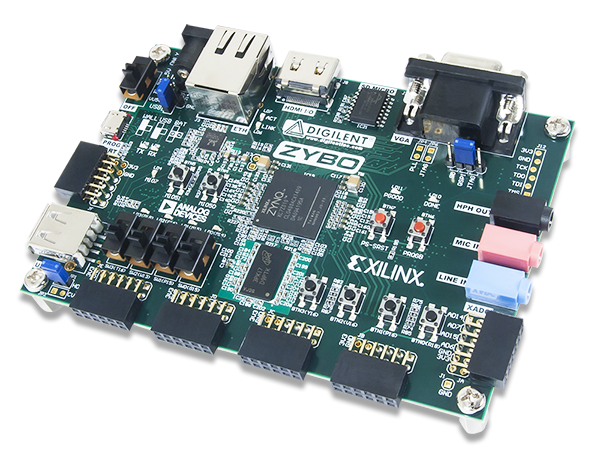
\includegraphics[width=\textwidth,height=\textheight,keepaspectratio]{images/zybo.png}
		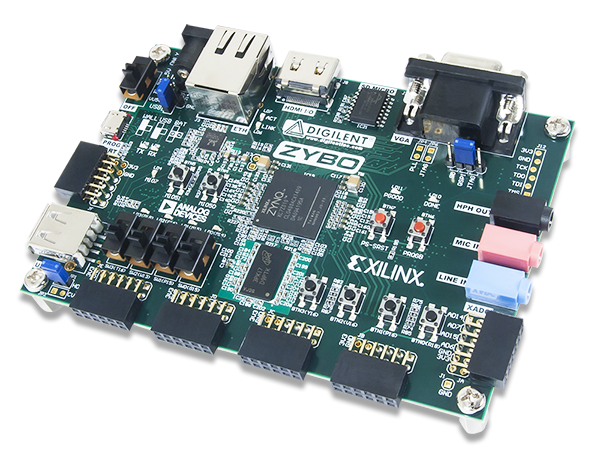
\includegraphics[width=8cm,height=\textheight,keepaspectratio]{images/zybo.png}
	\caption[]{Das Zybo mit dem Zynq-7000 SOC}
	\label{fig:zybo}
\end{figure}

